

\chapter{Introduction}



\noi A cipher consist of en encoder and a decoder. The algorithm behind the encoder and the decoder has to be public in order to ensure the integrity and the robustness of the cipher. The ciphers are typically  open source projects, reviewed by security experts.  \\

\subsection{Definitions}

\emph{Encoder : } $E : KxM \mapsto C$ \\
\emph{Decoder : } $D : KxC \mapsto M$ \\

\emph{Equality : } $ D(k, E(k,m) ) = m $ \\

E is often randomized whereas D is always deterministic.

\begin{figure}[ht!]
	\centering
		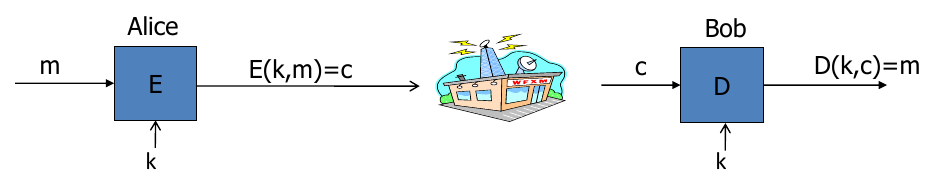
\includegraphics[width=0.7\textwidth]{tata}
	\caption{Cipher}
	\label{fig:Cipher}
\end{figure}

\noi A common mistake is to think that an ad-hoc crypto algorithm with closed source is safer than open source standards : the big problem with closed source algorithms is when they are breached, the user does not know.\\


\noi Uses of crypto : 
\begin{itemize}
		\item Secure communication : private conversations without eavesdropping 
		\item Digital signatures : secure identification (no tampering)
		\item Anonymous communication : secure and private communication without any of the participants know the identity of the others  
		\item Anonymous computation : outsourcing computation without giving the purpose of the calculus to the contractor (e.g. Amazon w3s)\\
\end{itemize}

\subsection{Trusted authority}

\noi A mecanism to ensure confidentiality is to outsource the task to a 3-rd party which has credibility and trust, like when we give our last will to a exterior person which does not have any involvement with the family(typically a \emph{notaire}).

\noi However, the trusted authority solution - like any centralized mecanism -  creates a single point of failure, so the trusted authority might not be always a good solution. \\

\emph{Theorem} : Any computation done by trusted auth can be done without it.\\


\subsection{ Zero proof of knowledge }
Aim of crypto : prove that, under a certain threat vector, forge the signature comes to solve a NP-problem.

\subsection{History of ciphers}

\noi cryptology is an ancient matter : all sorts of encoding scheme has been invented throughout History. \\
\emph{Definition :} $E(k,m)$ is the encryption of message $m$ using key $K$. (the key always first ) \\

\subsubsection{Substitution cipher }
The substitution cipher ( also called Julius code in its weak form ) is a simple encoder, yet relatively effective : the key $K$ is a bijective map between two alphabets. For example, $A$ becomes $D$, $B$ becomes $J$, etc.\\
The encryption is simply the substitution of every letter in the message $m$ by its counterpart in the map $K$.\\
The substitution cipher is however breakable only by looking at the ciphertexts ($=$ encryption of messages). The study of the letters' frequencies in the ciphertexts can give huge informations on the map $K$. In English, the letter $e$ is the most used so, by looking which letter is the most used in the ciphertexts, we can give a retty good guess of the subsitution of $e$.\\

\subsubsection{Vigener cipher }
breakable if we know the size of the
cipher => substation cipher.\\

\subsubsection{Enigma }
: substitution rotating cipher\\








